\documentclass[12pt]{exam}
\usepackage{amsthm}
\usepackage{libertine}
\usepackage[utf8]{inputenc}
\usepackage[margin=1in]{geometry}
\usepackage{amsmath,amssymb}
\usepackage{multicol}
\usepackage[shortlabels]{enumitem}
\usepackage{siunitx}
\usepackage{cancel}
\usepackage{graphicx}
\usepackage{listings}
\usepackage{tikz}
\usepackage{booktabs}

%\printanswers % Comment out to hide answers 
\CorrectChoiceEmphasis{\color{red}\bfseries\itshape}

\newcommand{\class}{\textbf{EC 380}} % This is the name of the course 
\newcommand{\examnum}{\textbf{Practice Final}} % This is the name of the assignment
\newcommand{\examdate}{\textbf{}} % This is the due date
\newcommand{\timelimit}{}
\addpoints % Allows to add points up to include table at end of document

\pagestyle{headandfoot} % Fancy equivalent for exam documentclass
\firstpageheadrule % Horizontal bar in first page
\runningheadrule % Horizontal bar in rest of pages
\firstpageheader{\class}{\examnum}{\examdate} % 1st page header content
\firstpagefooter{Points earned: \makebox[1in]{\hrulefill} / \pointsonpage{\thepage} points}{}{\thepage\ of \numpages} % 1st page footer content
\runningheader{\class}{\examnum}{\examdate} % Rest of pages header content
\runningfooter{Points earned: \makebox[1in]{\hrulefill} / \pointsonpage{\thepage} points}{}{\thepage\ of \numpages} % Rest of pages footer content
\bracketedpoints % Puts points per question inside brackets instead of parenthesis 


\title{Practice Final Exam}
\author{EC 380 - International Economic Issues}
\date{Winter 2025}

\begin{document}

%-------------------------------------------------------------------------------
\begin{coverpages}

\maketitle

\begin{center}
\fbox{\fbox{\parbox{5.5in}{\centering
Give every question your best attempt. \\
Best of luck. \\
You got this!
}}}\end{center}
\vspace{2cm}
\makebox[0.6\textwidth]{Name:\enspace\hrulefill}
\makebox[0.35\textwidth]{95\#:\enspace\hrulefill}

\vspace{1cm}
\noindent
The maximum amount of points on this exam is 90 points. 
You have a total of 2hrs (120 minutes) to complete the exam. 
The only items allowed on your desk at any time are a pen and/or pencil, scratch paper, a 3x5 note card, and a calculator. 
Everything else must be stored in your bag underneath your desk. 
Any form of cheating will result on a zero on the exam.\\

\noindent There are three sections to be completed:

\begin{itemize}
    \item \textbf{Multiple Choice:} 4 Questions
    \item \textbf{Short Answer Questions:} 2 Questions
    \item \textbf{Multi-Part Analysis Questions:} 1 Question (3 parts)
\end{itemize}

\noindent Point totals and question specific instructions are listed for each section.
Please ask for clarification if a question is not clear to you.\\

\noindent The exam packet is a total of \numpages $\,$ pages.
There are 6 pages of the exam + 2 pages for scratch paper.

\noindent \textbf{Please verify you have all \numpages $\,$ in your exam. If you do not, let me know immediately.}

\noindent 

\end{coverpages}
%-------------------------------------------------------------------------------

%-------------------------------------------------------------------------------
\section*{Multiple Choice}
Circle or "X" the answer you think most correctly answers the following questions. 
If you mark a choice and would like to change it, \textbf{clearly indicate which one is your correct answer}. 
%-------------------------------------------------------------------------------
\begin{questions}

\question[4] % Question 1
Suppose a given country maintains a highly unsustainable current account deficit and exhibits all the signs of a looming economic crash. 
Why might neighboring countries and those invested in said country be concerned about this?
    \begin{choices}
        \choice They have no reason to be concerned. 
        \correctchoice They face greater risk of negative spillovers
        \choice They care about their neighbors
        \choice It depends on whether the neighboring countries are in a deficit 
    \end{choices}
\vspace*{\stretch{1}}

\question[4] % Question 2
Consider the case in where the USD-EUR exchange rate is equal to 1.05. 
What is the value of the \textbf{EUR-USD} exchange rate?
    \begin{choices}
        \choice 0.05
        \choice 1.95  
        \correctchoice 0.95
        \choice Need to know more about the demand and supply of EUR in the US
    \end{choices}
\vspace*{\stretch{1}}

\question[4] % Question 4
Recall the formula to calculate the payoff of a bond: $P \times (1 + i)^{n}$. 
What does the $n$ stand for?
    \begin{choices}
        \choice The annual dividend yield of the bond
        \choice The current market price of the bond
        \correctchoice Years the bond accrues interest before maturing
        \choice The amount of bonds purchased
    \end{choices}
\vspace*{\stretch{1}}

\question[4] % Question 5
If a country is labeled as a net borrower, what does this suggest about the value/sign of the \textbf{current account balance}?
    \begin{choices}
        \choice The current account balance is zero
        \choice Current account balance does not account for borrowing/lending
        \correctchoice The current account balance is likely negative
        \choice The current account balance is likely positive
    \end{choices}
\vspace*{\stretch{1}}

%-------------------------------------------------------------------------------
\newpage
\section*{Short Answer}
Answer the following questions to the best of your ability.
For full credit, show all of your work and clearly indicate your final solution for each party by circling the answer.
%-------------------------------------------------------------------------------
\question[5]
Why are multinational firms particularly exposed to exchange rate risk?
How do can they hedge themselves away from this risk?
\begin{solution}
    \begin{itemize}
        \item Their contracts are defined in nominal currency amounts which carry uncertainty across time due to exchange rate volatility.
        \item They can hedge by using future contracts/forward exchange rates which set the future exchange rate at the time of signing.
    \end{itemize}
\end{solution}
\vspace*{\stretch{1}}
%-------------------------------------------------------------------------------
\question[5] 
What did \textbf{NAFTA} do to address immigration between the US and Mexico?

\begin{solution}
    
\end{solution}
\vspace*{\stretch{1}}

%-------------------------------------------------------------------------------
\question[5]
Write the mathematical formula for the \textbf{interest rate parity relationship}.
Identify each variable and explain the relationship intuitively.
\begin{solution}
    \begin{align*}
        i - i^{*} = \dfrac{(F - R)}{R}
    \end{align*}
    \begin{itemize}
        \item $i$ is the \textbf{home country} interest rate
        \item $i^{*}$ is the \textbf{foreign country} interest rate
        \item $F$ is the future exchange rate
        \item $R$ is the current/spot exchange rate
    \end{itemize}
    This relationship shows that the difference between countries' interest rates should be equal to the expected chagne of the exchange rate. 
    This equality eliminates/minimizes arbitrage opportunities.
\end{solution}
\vspace*{\stretch{1}}

%-------------------------------------------------------------------------------
\newpage
\section*{Multi-Part Analysis}
Answer the following questions to the best of your ability.
For full credit, \textbf{show all of your work and clearly indicate your final solution} for each part by circling the answer.
%-------------------------------------------------------------------------------
\question
Consider the following demand and supply curves of foreign currency, where \textbf{ExR} represents the local to foreign currency exchange rate.
\textbf{FC} represents the units of foreign currency reserves held in the ``local" economy.

\begin{align*}
    \text{Demand:} \text{ ExR} = 180 - 0.290FC \;\;\; ; \;\;\; \text{Supply:} \text{ ExR} = 50 + 0.251FC
\end{align*}

\begin{parts}
    \part[10]
    What is the \textbf{market clearing rate of exchange and level of foreign currency reserves}?
    \begin{solution}
        Solve by setting Demand equal to Supply
        \begin{multicols}{2}
            \begin{align*}
                \text{Demand} &= \text{Supply} \\
                180 - 0.290FC &= 50 + 0.251FC \\
                130 &= 0.541FC \\
                FC &\approx 240.30 
            \end{align*}
            
            \begin{align*}
                \text{ExR} &= 50 + 0.251(240.30) \\
                \text{ExR} &\approx 110.32
            \end{align*}
        \end{multicols}
    \end{solution}
    \vspace*{\stretch{2}}
    \part[5]
    Consider a case in which a large cache of foreign currency is discovered following an audit of local steel factories, causing foreign currency reserves to increase in supply by 40 units. 
    This increase in supply is represented on the supply curve as $S' = S - 40$. 
    What are the \textbf{new exchange rate and currency reserve values}?
    \begin{solution}
        We re-write the Supply equation by simply subtracting 40 from it and solve as we did previously
        \begin{multicols}{2}
            \begin{align*}
                \text{Demand} &= \text{New Supply} \\
                180 - 0.290FC &= 50 + 0.251FC - 40 \\
                180 - 50 + 40 &= 0.541FC \\
                170 &= 0.541FC \\
                FC &\approx 314.23
            \end{align*}

            \begin{align*}
                \text{ExR} &= 10 + 0.251(314.23) \\
                \text{ExR} &\approx 88.87
            \end{align*}
        \end{multicols}

    \end{solution}
    \vspace*{\stretch{2}}
    \newpage
    \part[10]
    Draw a graph that represents the supply and demand of a foreign currency.
    In this graph, show the dynamics found in the previous steps. 
    \textbf{Label everything properly. Since you have found equilibrium values, be sure to use those values.}
    \vspace{1cm}
    \begin{figure}[hb]
        \centering
        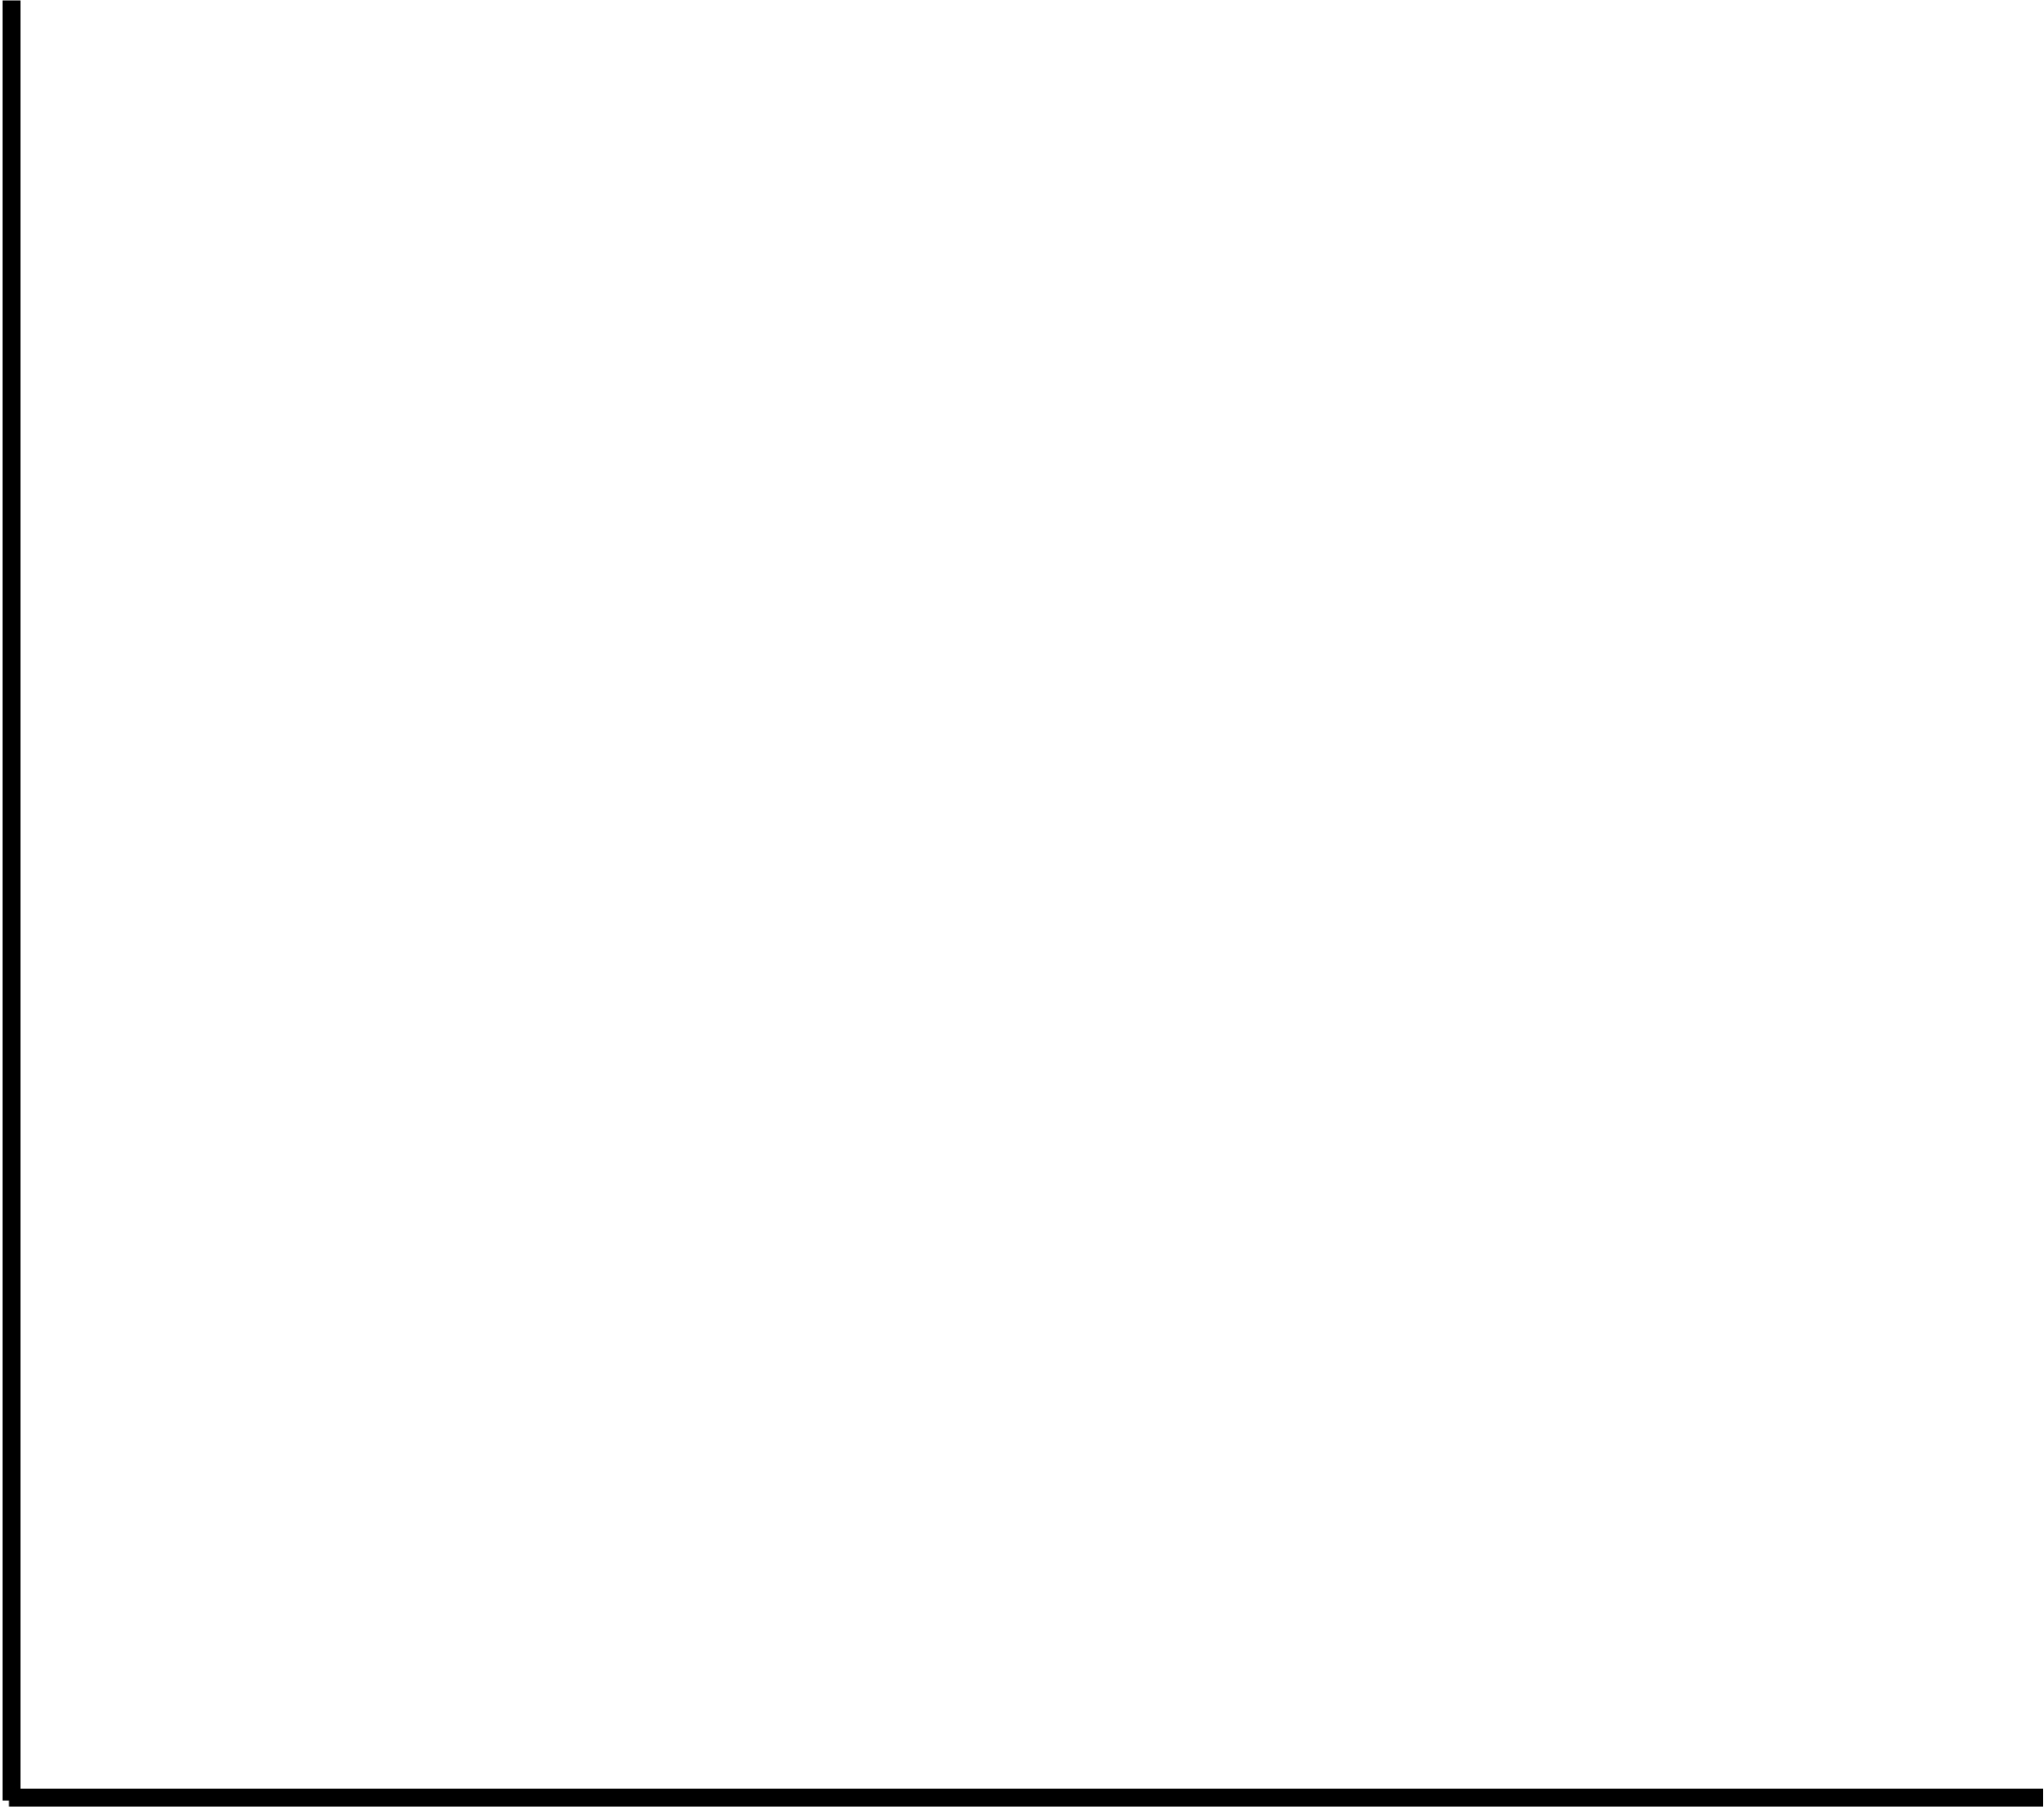
\includegraphics[width=1\linewidth]{images/empty-graph.png}
    \end{figure}
\end{parts}
\end{questions}

%-------------------------------------------------------------------------------
\end{document}